% Compilar desde esta carpeta; estilo de la clase del jueves 26.
\documentclass[10pt,aspectratio=169,xcolor={dvipsnames}]{beamer}
\usepackage[utf8]{inputenc}
\usepackage[T1]{fontenc}
\usepackage{lmodern}
\usepackage[spanish,es-nodecimaldot]{babel}
\usepackage{amsmath,amssymb,bm}
\usepackage{graphicx,booktabs,tikz,listings}
\usetikzlibrary{arrows.meta,positioning,calc}
\graphicspath{{figuras/}}

% Paleta, títulos y recuadros del material DL_MRI_class.
\definecolor{fondo}{RGB}{18,49,90}
\definecolor{verde}{HTML}{087F6B}
\definecolor{naranja}{HTML}{D65324}
\setbeamercolor{normal text}{fg=fondo,bg=white}
\setbeamercolor{math text}{fg=black!75}
\setbeamercolor{structure}{fg=fondo}
\setbeamercolor{frametitle}{fg=fondo,bg=white}
\setbeamercolor{bottombox}{fg=fondo,bg=white}
\setbeamercolor{lgraybox}{fg=fondo,bg=gray!10}
\setbeamercolor{yellowbox}{fg=fondo,bg=yellow!17}
\setbeamercolor{greenbox}{fg=fondo,bg=verde!10}
\setbeamercolor{orangebox}{fg=fondo,bg=naranja!10}
\setbeamercolor{section title}{fg=fondo,bg=white}
\setbeamercolor{itemize item}{fg=fondo}
\setbeamertemplate{itemize items}[circle]
\setbeamertemplate{navigation symbols}{}
\setbeamersize{text margin left=8mm,text margin right=8mm}
\setbeamertemplate{frametitle}{\vspace{2mm}\color{fondo}\bfseries\insertframetitle\par\vspace{-2mm}\rule{\textwidth}{0.4pt}}
\setbeamertemplate{footline}{%
    \leavevmode\hbox{%
    \begin{beamercolorbox}[wd=.23\paperwidth,ht=2.5ex,dp=1ex,center]{bottombox}
        \insertshortauthor
    \end{beamercolorbox}%
    \begin{beamercolorbox}[wd=.46\paperwidth,ht=2.5ex,dp=1ex,center]{bottombox}
        \insertshorttitle
    \end{beamercolorbox}%
    \begin{beamercolorbox}[wd=.31\paperwidth,ht=2.5ex,dp=1ex,right]{bottombox}
        \insertshortdate\hspace{1.5em}\insertframenumber/\inserttotalframenumber\hspace{2ex}
    \end{beamercolorbox}}\vskip2pt}
\newcommand{\tcg}[1]{\textcolor{verde}{#1}}
\newcommand{\tcr}[1]{\textcolor{naranja}{#1}}
\newenvironment{caja}[1][lgraybox]{\begin{beamercolorbox}[sep=0.7em,wd=\linewidth]{#1}}{\end{beamercolorbox}}
\newcommand{\actividad}[2]{\begin{caja}[yellowbox]\textbf{#1}\par\smallskip #2\end{caja}}
\newcommand{\R}{\mathbb{R}}
\DeclareMathOperator*{\argmin}{arg\,min}
\lstset{language=Python,basicstyle=\ttfamily\small,keywordstyle=\color{fondo}\bfseries,
    commentstyle=\color{verde},stringstyle=\color{naranja},showstringspaces=false,
    columns=fullflexible,keepspaces=true,frame=none,aboveskip=0.5em,belowskip=0.5em}
\setbeameroption{hide notes}
% Para una versión docente intercalada, cambiar la línea anterior por:
% \setbeameroption{show notes}
\AtBeginSection[]{%
    \begin{frame}[plain]
        \vfill
        {\small APRENDIZAJE AUTOMÁTICO INICIAL\par}
        \vspace{5mm}
        {\LARGE\bfseries\insertsection\par}
        \vspace{3mm}{\color{naranja}\rule{0.25\textwidth}{1.2pt}}
        \vfill
    \end{frame}}

\title[Clase 13]{\bfseries Perceptrón sigmoide y multiclase}
\subtitle{De una predicción numérica a probabilidades de clase}
\author[E. Cueva]{Evelyn Cueva J.}
\institute{Aprendizaje Automático Inicial · Ciencia de Datos}
\date[30 nov. 2026]{Lunes 30 de noviembre de 2026}

\begin{document}
\begin{frame}[plain]
    \vspace{6mm}{\small CLASE 13\par}\vspace{6mm}
    {\LARGE\bfseries\inserttitle\par}\vspace{3mm}
    {\color{fondo}\rule{0.92\textwidth}{1pt}}\par
    {\large\insertsubtitle\par}\vspace{8mm}
    \insertauthor\par\smallskip{\small\insertinstitute\par}\vspace{3mm}
    {\small\insertdate\par}\vfill
\end{frame}
\begin{frame}{Del jueves al lunes: ¿qué cambia al clasificar?}
\begin{itemize}
\item El jueves: $\hat y=\bm w^\top\bm x+b$ predice una cantidad.
\item Hoy: queremos decidir a qué clase pertenece una observación.
\item Conservamos pesos, sesgo, pérdida y actualizaciones por gradiente.
\end{itemize}\begin{caja}[yellowbox]
Pregunta inicial: ¿cómo penalizar una clasificación equivocada con mucha confianza?
\end{caja}

\note{}
\end{frame}

\begin{frame}{Objetivos y recorrido}
\begin{itemize}
\item Relacionar puntaje, probabilidad y decisión.
\item Derivar el gradiente de sigmoide con entropía cruzada binaria.
\item Extender la salida a varias clases con softmax.
\item Interpretar y experimentar con los dos notebooks de referencia.
\end{itemize}
\note{}
\end{frame}

\section{Clasificación binaria: de un puntaje a una decisión}
\begin{frame}{Observaciones, entradas y etiquetas}
\centering
\begin{tabular}{cccc}\toprule
Observación & $x_1$ & $x_2$ & $y$\\\midrule
1 & 0.2 & 1.1 & 0\\2 & 1.4 & 0.3 & 1\\3 & 0.8 & 0.7 & 1\\\bottomrule
\end{tabular}\par\bigskip
\raggedright Datos ilustrativos: cada fila tiene dos entradas y una etiqueta conocida.
\[\bm x\in\R^2,\quad y\in\{0,1\},\quad z=w_1x_1+w_2x_2+b.\]
El puntaje $z$ puede tomar cualquier valor real; todavía no es una probabilidad.
\note{}
\end{frame}

\begin{frame}{Sigmoide: convertir el puntaje en probabilidad}
\[p=\sigma(z)=\frac{1}{1+e^{-z}},\qquad 0<p<1.\]\begin{itemize}
\item Interpretamos $p$ como una estimación de $P(y=1\mid\bm x)$.
\item Con umbral $\tau=0.5$: predecimos clase 1 si $p\geq0.5$.
\item La frontera de decisión cumple $z=0$: sigue siendo lineal.
\end{itemize}\begin{caja}[greenbox]
Una activación no lineal en la salida no crea, por sí sola, una frontera curva.
\end{caja}

\note{La interpretación probabilística corresponde al modelo de Bernoulli entrenado con BCE; no garantiza calibración perfecta. El umbral puede elegirse con validación según los costes de error.}
\end{frame}

\begin{frame}{Forma de la sigmoide y coste de equivocarse}
\centering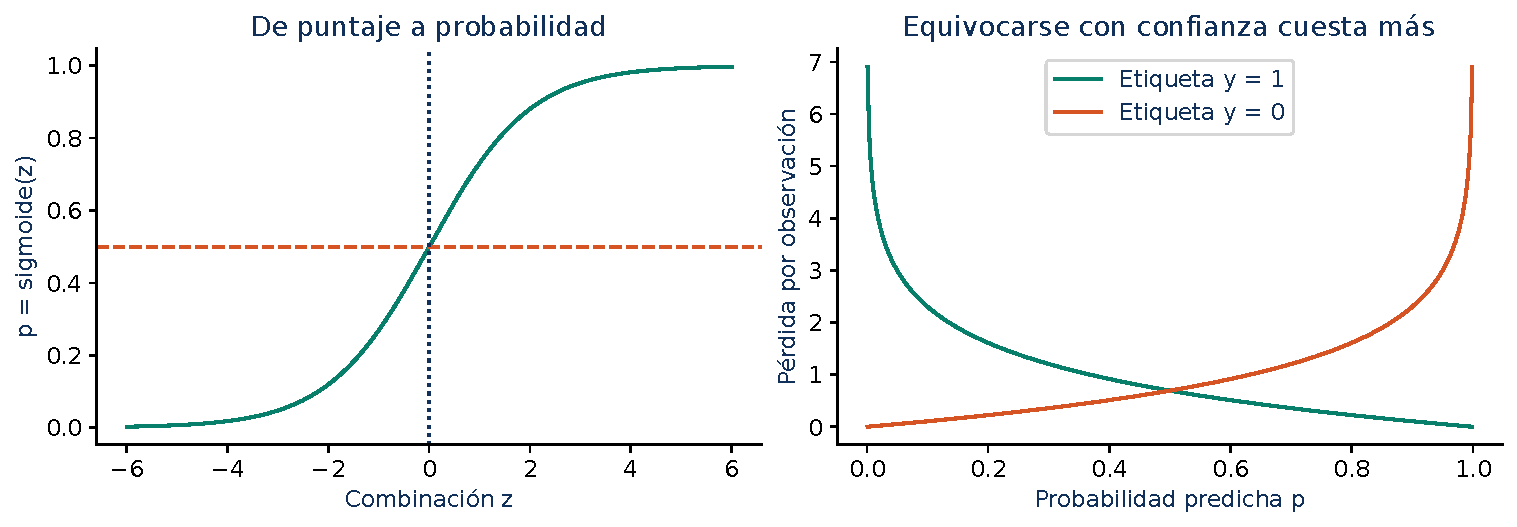
\includegraphics[width=\linewidth,height=4cm,keepaspectratio]{sigmoide_perdida.pdf}\par\medskip
aggedright\small Para $y=1$, acercar $p$ a 0 aumenta mucho la pérdida; para $y=0$, ocurre al acercarlo a 1.
\note{}
\end{frame}

\begin{frame}{La pérdida debe corresponder a la tarea}

\begin{caja}[yellowbox]
\textbf{Entropía cruzada binaria (BCE)}
\[\ell(y,p)=-y\log p-(1-y)\log(1-p),\qquad
\mathcal L=\frac1N\sum_i\ell(y_i,p_i).\]
\end{caja}
Si $y=1$: $p=0.9\Rightarrow\ell\approx0.105$;
$p=0.1\Rightarrow\ell\approx2.303$.\par\bigskip
La exactitud cuenta aciertos; la pérdida también distingue la confianza.
\actividad{Antes de calcular}{¿Dos modelos con la misma exactitud pueden tener distinta BCE?}
\note{Usamos logaritmos naturales. Una pérdida baja no sustituye la evaluación con datos nuevos.}
\end{frame}

\begin{frame}{Regla de la cadena: de la pérdida al puntaje}

\[\frac{\partial\ell}{\partial p}=\frac{p-y}{p(1-p)},
\qquad\frac{\partial p}{\partial z}=p(1-p).\]
\begin{caja}[greenbox]\centering
\[\frac{\partial\ell}{\partial z}
=\frac{\partial\ell}{\partial p}\frac{\partial p}{\partial z}=p-y.\]
\end{caja}
\[\nabla_{\bm w}\mathcal L=\frac1N\sum_i(p_i-y_i)\bm x_i,
\qquad\partial_b\mathcal L=\frac1N\sum_i(p_i-y_i).\]
El error $p-y$ se combina con cada entrada para ajustar su peso.
\note{}
\end{frame}

\begin{frame}{Un paso a mano: comprobar la dirección}

Un dato: $x=2$, $y=1$. Inicio: $w=0$, $b=0$; $\eta=0.1$.
\begin{align*}
z&=0,&p&=0.5,&\ell&=\log2\approx0.693,\\
\partial_w\ell&=(0.5-1)2=-1,&\partial_b\ell&=-0.5,\\
w_{\rm nuevo}&=0.1,&b_{\rm nuevo}&=0.05.
\end{align*}
\[z_{\rm nuevo}=0.25,\quad p_{\rm nuevo}\approx0.562,
\quad\ell_{\rm nueva}\approx0.576.\]
\actividad{Interpreta}{La etiqueta es 1: ¿por qué era razonable aumentar la probabilidad?}
\note{}
\end{frame}

\begin{frame}{Notebook binario: dónde mirar}
\begin{itemize}
\item \texttt{13-1-Perceptron-Sigmoide.ipynb}: 100 datos, dos variables, dos centros.
\item Celdas 7 y 10: datos y clase de Python; celda 12: entrenamiento.
\item El sesgo se integra añadiendo una columna de unos: $\tilde X=[\bm1,X]$.
\item El primer peso es el sesgo; el resto multiplica las entradas.
\end{itemize}
\note{Numeración posicional de celdas desde 1 en el archivo original. Entrenar desde el comienzo; las dos clases Perceptron de los dos notebooks no son la misma implementación.}
\end{frame}

\begin{frame}[fragile]{Una implementación numéricamente estable}
\begin{lstlisting}
z = X_bias @ w
p = 1 / (1 + np.exp(-np.clip(z, -500, 500)))
loss = np.mean(np.logaddexp(0, z) - y * z)
grad = X_bias.T @ (p - y) / len(y)
w = w - lr * grad
\end{lstlisting}
\begin{caja}[greenbox]
BCE calculada desde los logits: evita evaluar directamente el logaritmo de 0.
\end{caja}

\note{Adaptación propuesta a la celda 10, no modificación del original. X_bias contiene los unos. Para rangos extremos puede emplearse una sigmoide estable por ramas. El recorte de aquí evita overflow para rangos habituales de la demostración.}
\end{frame}

\begin{frame}{Ejemplo visual: frontera y entrenamiento}
\centering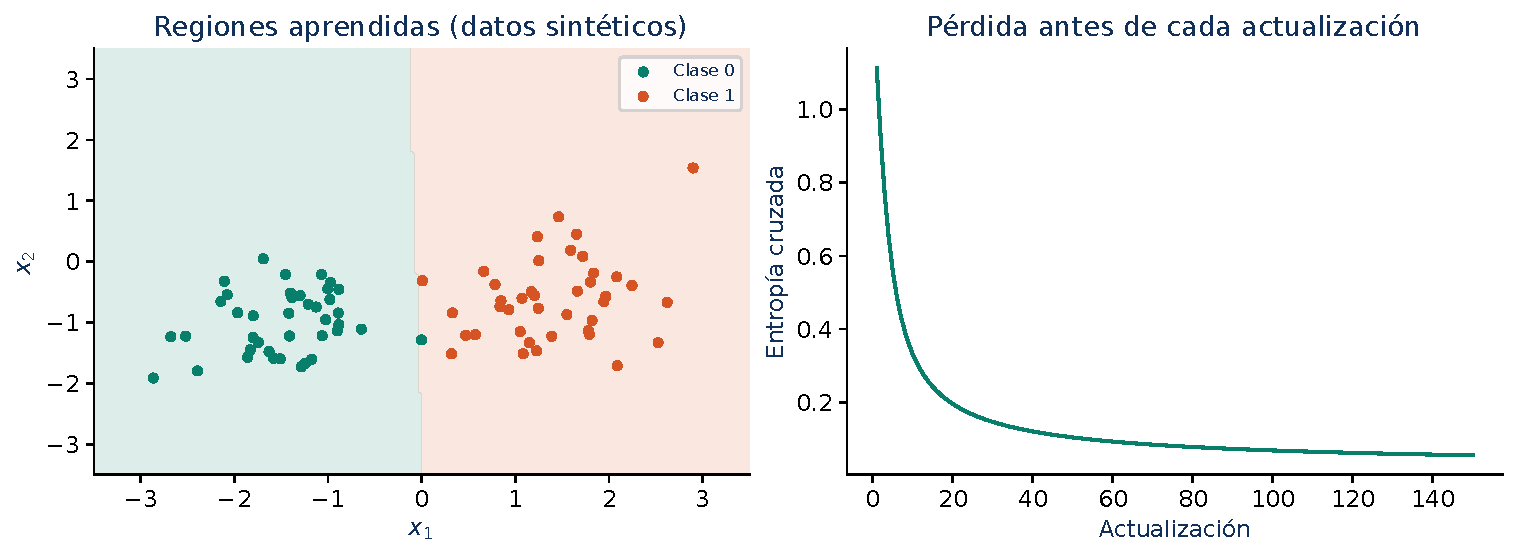
\includegraphics[width=\linewidth,height=4cm,keepaspectratio]{clasificacion_2.pdf}\par\medskip
aggedright\small Ajuste NumPy reproducible sobre datos sintéticos: dos salidas softmax, equivalente a una frontera logística binaria.
\note{La figura no es una ejecución del notebook: usa 80 datos sintéticos y 150 pasos de lote completo. Diferenciar equivalencia de la familia de modelos y trayectoria numérica exacta.}
\end{frame}

\begin{frame}{Actividad: cambiar una sola decisión}
\begin{itemize}
\item Conservar datos e inicialización; comparar $\eta=0.1,0.01,0.001$.
\item Registrar pérdida final y exactitud usando umbral 0.5.
\item Aumentar la dispersión de los datos y observar el solapamiento.
\end{itemize}
\note{En el notebook original la pérdida se guarda antes del paso y el peso después. Para una animación sincronizada, registrar ambos antes o ambos después. No atribuir pérdida y frontera de un frame a los mismos parámetros sin corregir ese desfase.}
\end{frame}

\section{Varias clases: una salida que compite}
\begin{frame}{Tres clases mutuamente excluyentes}

Ejemplo: asignar una observación a una de tres categorías.
\[\bm z=W^\top\bm x+\bm b,\quad
\bm x\in\R^d,\ W\in\R^{d\times K},\ \bm b\in\R^K.\]
\begin{caja}\textbf{Un puntaje por clase.}
Cada columna de $W$ tiene los pesos de una clase; cada clase tiene su sesgo.\end{caja}
Para $d=2$, $K=3$: hay $2\times3+3=9$ parámetros.
\actividad{Predice}{Si los puntajes son $(2,1,0)$, ¿qué clase debería tener mayor probabilidad?}
\note{}
\end{frame}

\begin{frame}{Softmax: probabilidades que suman uno}

\[p_k=\frac{e^{z_k}}{\sum_{j=1}^K e^{z_j}},\quad
\sum_kp_k=1,\quad\hat c=\arg\max_kp_k.\]
\[\bm z=(2,1,0)\quad\Longrightarrow\quad
\bm p\approx(0.665,0.245,0.090).\]
\begin{caja}[yellowbox]
Softmax acopla las salidas: cambiar un puntaje modifica todas las probabilidades.
\end{caja}
Se usa para clases excluyentes; varias etiquetas simultáneas requieren otro planteamiento.
\note{}
\end{frame}

\begin{frame}{La etiqueta y su pérdida multiclase}

Para la clase verdadera 1 (índices 0, 1, 2): $\bm y=(0,1,0)$.
\[\ell(\bm y,\bm p)=-\sum_k y_k\log p_k=-\log p_1.\]
Con $\bm p=(0.665,0.245,0.090)$, $\ell\approx1.407$.
\par\bigskip
\textbf{One-hot:} vector con un 1 en la clase verdadera.
\par\medskip
\textbf{Etiqueta entera:} índice de clase; puede usarse con una pérdida categórica dispersa.
\actividad{Interpreta}{¿Qué probabilidad debe aumentar para reducir esta pérdida?}
\note{}
\end{frame}

\begin{frame}{Gradiente de softmax con entropía cruzada}

\[\frac{\partial p_j}{\partial z_k}=p_j(\delta_{jk}-p_k),
\qquad \frac{\partial\ell}{\partial z_k}=p_k-y_k.\]
Con matrices por filas: $X\in\R^{N\times d}$, $P,Y\in\R^{N\times K}$.
\[\nabla_W\mathcal L=\frac1N X^\top(P-Y),\qquad
\nabla_{\bm b}\mathcal L=\frac1N\sum_i(P_i-Y_i).\]
\begin{caja}[greenbox]La estructura sigue siendo: error de salida, entradas y actualización.\end{caja}
\note{Mostrar la derivada de softmax como Jacobiano, no como K sigmoides independientes. En la fórmula de sesgo el resultado se interpreta como vector de K componentes.}
\end{frame}

\begin{frame}[fragile]{Notebook multiclase: seguir las dimensiones}
\begin{lstlisting}
# X_bias: (N, d+1); W: (d+1, K)
z = X_bias @ W
z = z - z.max(axis=1, keepdims=True)
p = np.exp(z)
p = p / p.sum(axis=1, keepdims=True)
Y = np.eye(K)[y]
grad = X_bias.T @ (p - Y) / len(y)
W = W - lr * grad
\end{lstlisting}

\note{13-2-Perceptron-Multiclase.ipynb: celdas 7, 10 y 12. La sustracción del máximo mejora estabilidad sin alterar las probabilidades. Aquí W incluye el sesgo como primera fila.}
\end{frame}

\begin{frame}{Regiones de decisión multiclase}
\centering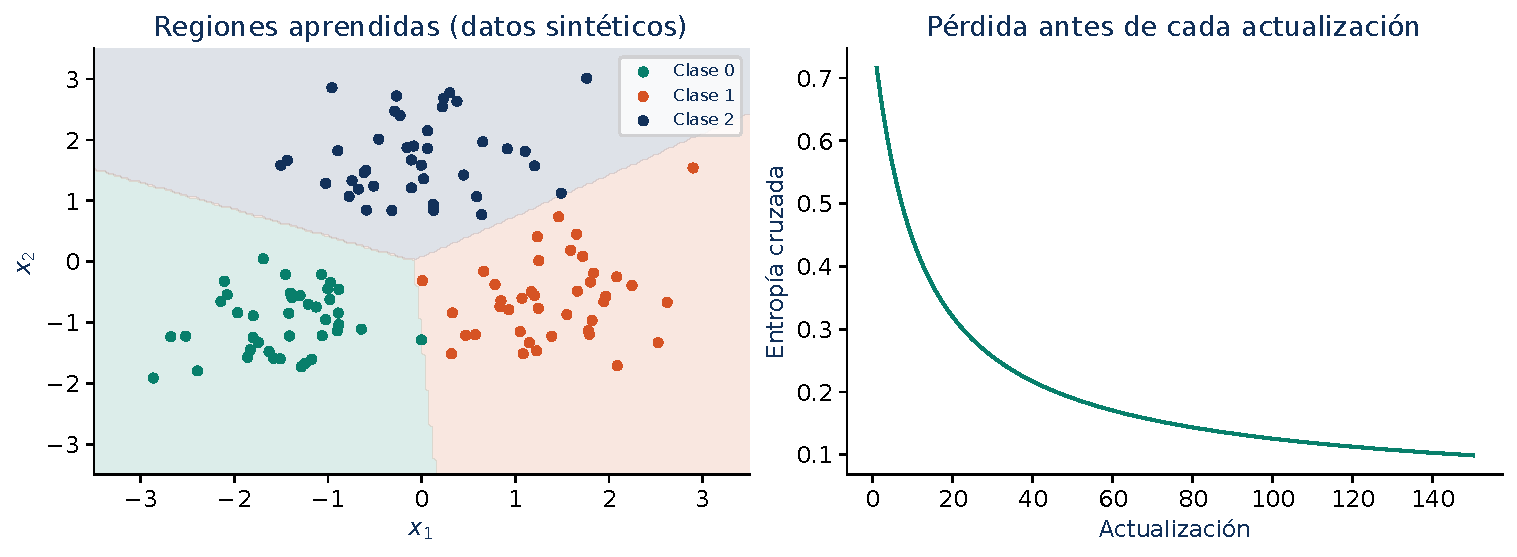
\includegraphics[width=\linewidth,height=4cm,keepaspectratio]{clasificacion_3.pdf}\par\medskip
aggedright\small Las regiones compiten mediante $\arg\max$; la frontera entre dos puntajes afines es lineal.
\note{Ajuste NumPy generado con el script de figuras, 120 observaciones sintéticas, tres clases; no son resultados del notebook histórico.}
\end{frame}

\begin{frame}{Verificación: elegir salida, pérdida y decisión}
\centering\small
\begin{tabular}{llll}\toprule
Tarea & Salida & Pérdida & Decisión\\\midrule
Regresión & Identidad & MSE & Valor numérico\\
Dos clases & Sigmoide & BCE & Umbral\\
$K$ clases excluyentes & Softmax & CE categórica & $\arg\max$\\\bottomrule
\end{tabular}\par\bigskip\raggedright
\actividad{Explica sin código}{¿Por qué tres sigmoides independientes no equivalen a softmax?}
\note{}
\end{frame}

\begin{frame}{Resumen y puente al martes}
\begin{itemize}
\item La activación de salida y la pérdida dependen de la tarea.
\item Con sigmoide+BCE y softmax+CE, el gradiente respecto al puntaje es $p-y$.
\item Una sola transformación afín mantiene fronteras lineales.
\item El martes: capas ocultas y activaciones no lineales para representar fronteras curvas.
\end{itemize}
\note{Lectura previa indicada por Clase13.pdf: qué es un framework y una API, y qué ofrecen PyTorch y TensorFlow. Preguntar qué aporta una capa oculta frente a cambiar solo el umbral.}
\end{frame}

\end{document}
